\section{Two-Phase Lagrangian Computation}

\subsection{What you Will Learn}

In this part of the tutorial, you will learn how to set-up, run, and post-process a Lagrangian two-phase flow simulation in \CS, and how to compare the numerical results with the experimental data of \cite{Arnason}.

\subsection{Create a case with ``copy-from'' feature}

In the following, only the modifications that need to be applied to the single phase flow set-up for the Lagrangian calculation are discussed.  Everything else remains as described previously. The information added for the Lagrangian particulates include the specification of the injection point for a particle size of $5\mu m$ diameter.

In order to {\bf avoid setting again} the RANS case as described in the previous section, the second case will be created using the ``copy-from'' feature. In \salome object browser, right click on the study name ``ARNASON'' and select \keys{Add case}. Then in the pop-up window, enter the name ``RANS\_rij\_SSG\_5M'' for example, toggle the option \keys{copy from existing case} and choose the first case directory ``RANS\_rij\_SSG''. Finally click on \keys{OK}.

\subsection{Setting up the Lagrangian Simulation}

Right click on the file setup.xml in the ‘RANS\_rij\_SSG\_5M/DATA’ directory which was just created in the object browser and select \keys{Open GUI}. Check that the directory of the case is ‘RANS\_rij\_SSG\_5M and the name of the file is setup.xml (if you see unnamed instead, close the file and repeat the instruction correctly).

You can now set-up the Lagrangian two-phase flow case.

\subsubsection{Setting up the Lagrangian Model}

\paragraph{Calculation Features:}

In the panel of the 'Calculation features' section, select ‘Frozen carrier flow’ in the drop down menu of the ‘Eulerian-Lagrangian model’ menu under the ‘Additional Features’ head as shown in \figurename~\ref{lag:flow_physics}.
%
\begin{figure}[H]
\centering
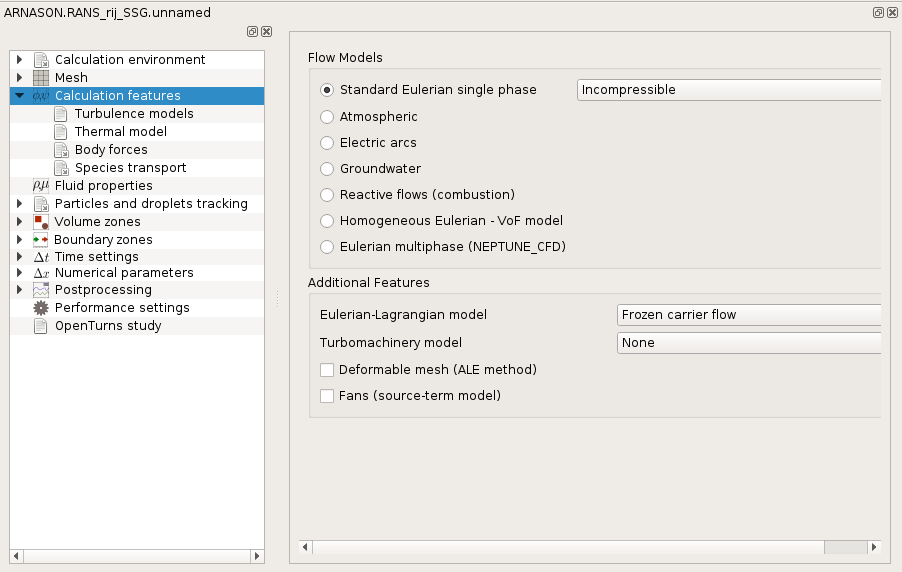
\includegraphics[width=0.8\textwidth]{\IMAGES/Part5_Lagrangian_computation/Lagr_calculation_features.png}
\caption{Selecting the flow physics.}\label{lag:flow_physics}
\end{figure}
%
\paragraph{Particles and Droplets Tracking:}

In the \menu{Particles and droplets tracking} folder that has now appeared in the GUI tree menu, click on the sub-folder \menu{Global settings} to display the panel.  By choosing 'Frozen carrier flow' in the previous section, the box ‘The continuous phase flow is a steady flow’ has been automatically ticked.  Leave all other settings in this panel at their default options.
%
\begin{figure}[H]
\centering
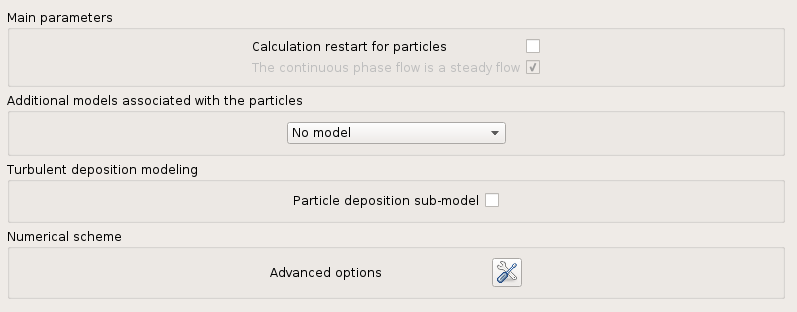
\includegraphics[width=0.8\textwidth]{\IMAGES/Part5_Lagrangian_computation/lagr_global_settings.png}
\caption{Global settings menu.}\label{lag:global_setting}
\end{figure}
%
Click on the ‘Advanced options’ icon to specify the numerical scheme, as shown in \figurename~\ref{lag:advanced_option}.  Let the other options at their default values. They should be ‘first order scheme’ for the ‘integration for the stochastic differential equations’ option and the ‘particle turbulent dispersion’ box should be ticked.
%
\begin{figure}[H]
\centering
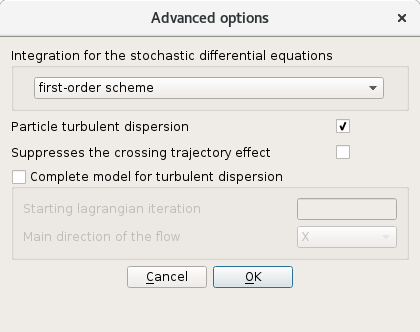
\includegraphics[width=0.6\textwidth]{\IMAGES/Part5_Lagrangian_computation/lagr_advanced_options.png}
\caption{Advanced options of the numerical scheme menu.}\label{lag:advanced_option}
\end{figure}
%
In the ‘Statistics’ sub-folder, select all parameters, as presented in \figurename~\ref{lag:statistics_menu}.  The number of particles present in the computational domain is constant after 150 iterations, hence the statistics are started after iteration 400 (cf. \figurename~\ref{lag:nb_particles} in \ref{lag:Resu_flow_field}).
%
\begin{figure}[H]
\centering
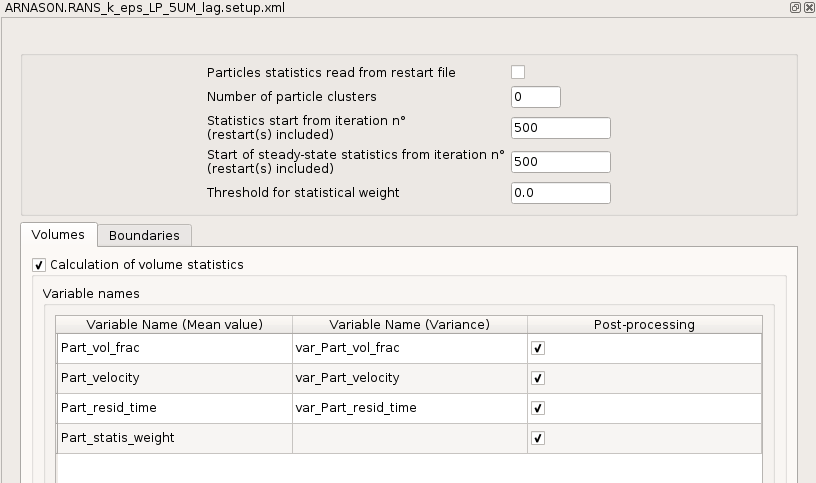
\includegraphics[width=0.8\textwidth]{\IMAGES/Part5_Lagrangian_computation/lagr_stat.png}
\caption{Statistics menu.}\label{lag:statistics_menu}
\end{figure}
%
In the panel of the \keys{Output control} sub-folder under the \keys{Postprocessing} section, ensure that the ‘Output listing at each time step’ is set to 1 for ``log frequency for particles''.  This will output particle information at every time step. In the \keys{Lagrangian solution control} subfolder, select all the options for the different variables to save.  The final set-up for this panel is shown in \figurename~\ref{lag:output_menu} and \figurename~\ref{lag:lagrangian_solution_control}.

\begin{figure}[H]
\centering
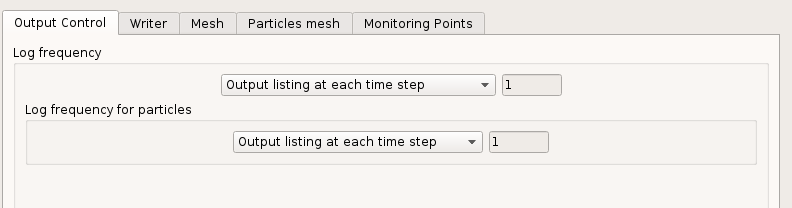
\includegraphics[width=0.8\textwidth]{\IMAGES/Part5_Lagrangian_computation/lagr_output_frequency.png}
\caption{Output menu.}\label{lag:output_menu}
\end{figure}

\begin{figure}[H]
\centering
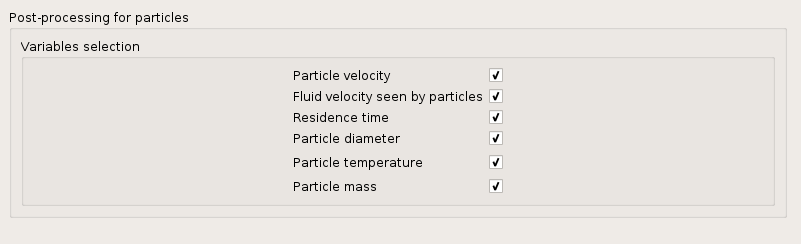
\includegraphics[width=0.8\textwidth]{\IMAGES/Part5_Lagrangian_computation/lagrangian_solution_control.png}
\caption{Solution controls.}\label{lag:lagrangian_solution_control}
\end{figure}

\paragraph{Volume zones}

In the experiments, the particles are injected further downstream of the pipe's inlet plane.  Therefore, we inject particles inside a volume section selected to contain the experiment's injection point. The injection will be defined below using the \textit{cs\_user\_lagr\_injection} and \textit{cs\_user\_lagr\_volume\_conditions} user functions but the zone has to be defined in the GUI.

In the section \menu{Volume zones > Definition of volume regions}, define a volume zone in which particles will be injected.
Name it ``particle\_injection'' and set ``injection'' in the selection criteria field to define it as shown on \figurename~\ref{lag:volume_zone_injection}.
Notice, that this zone has no ``nature'' defined for now, since its nature will be defined later in \textit{cs\_user\_lagr\_volume\_conditions}.
%
\begin{figure}[H]
\centering
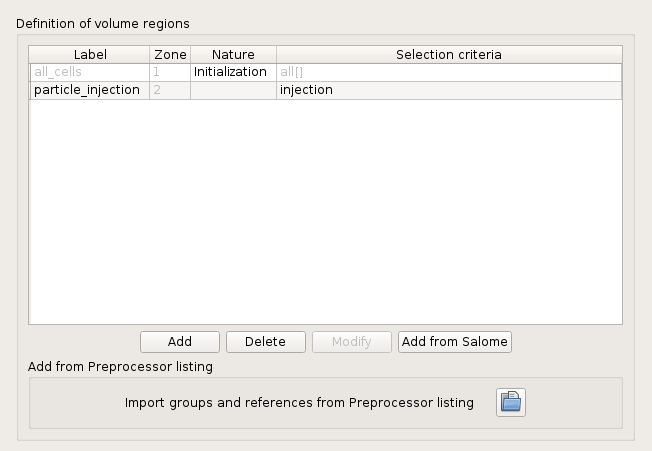
\includegraphics[width=0.8\textwidth]{\IMAGES/Part5_Lagrangian_computation/volume_zone_injection.png}
\caption{Definition of the volume zone in which particles will be injected.}\label{lag:volume_zone_injection}
\end{figure}
%

\paragraph{Particle Boundary Conditions:}

The next step is to set the ‘Particles boundary conditions’, which specify the boundary conditions for the particulate field.

Add the 'inlet' boundary in the \keys{Definition of boundary regions} sub-folder, but do not specify the boundaries further in this folder.  These will be specified for the particles in the \keys{Particles boundary conditions} sub-folder.

Go to the \keys{Particles boundary conditions} sub-folder and ensure that the type of ‘Particle-boundary interaction’ for the three boundary conditions inlet, outlet and wall are as follows:
%
\begin{itemize}
\item 'outlet': ‘Particles outlets’
\item ‘wall’: ‘Particles rebound’ $\Rightarrow$ particles bounce off walls without loss of energy
\item ‘inlet’: ‘Particles inlet’
\end{itemize}
%
This concludes the set-up of the specifics of the Lagrangian two-phase mode.  To complete the model in the GUI before moving to the required user coding, the numerical parameters should now be specified.

\subsubsection{Numerical Parameters}

In the \keys{Numerical Parameters} folder, leave all settings at the values set for the RANS calculation in the \keys{Global parameters} and \keys{Equation parameters} sub-folders.

In the \keys{Time step} panel specify a reference time step of 0.002s with 3000 iterations.  This will run the two-phase flow calculation for 2000 iterations, given that a \CS restart incudes the number of iterations previously completed.  The final set-up for this panel is shown in \figurename~\ref{lag:time_step_menu}.

\begin{figure}[H]
\centering
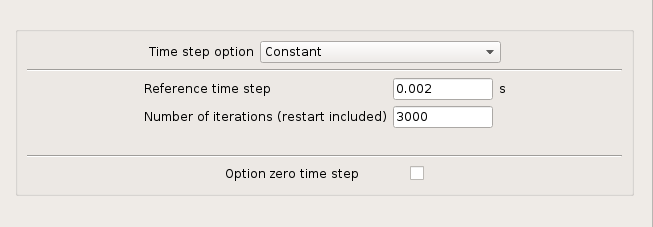
\includegraphics[width=0.8\textwidth]{\IMAGES/Part5_Lagrangian_computation/lagr_time_step.png}
\caption{Time step menu.}\label{lag:time_step_menu}
\end{figure}


\subsubsection{Start/Restart}

In the ‘Time settings’ section, go to the ‘Start/Restart’ sub-sectin to choose the restart file of the single phase fluid calculation.  Then tick the ‘Calculation on frozen velocity and pressure fields’ box as shown in \figurename~\ref{lag:start_restart_menu}, so that the particle field is injected on top of the previously calculated single-phase field.

\begin{figure}[H]
\centering
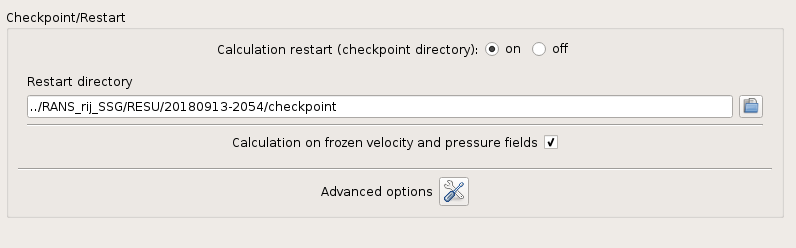
\includegraphics[width=0.8\textwidth]{\IMAGES/Part5_Lagrangian_computation/lagr_restart.png}
\caption{Start/restart menu.}\label{lag:start_restart_menu}
\end{figure}

The set-up of the two-phase flow model in the GUI is now complete.  If not already done, you should now save the 'xml' setup file.  Before you can run the simulation, user functions in \textit{cs\_user\_lagr\_particle.c}, \textit{cs\_user\_lagr\_volume\_conditions.c} and \textit{cs\_user\_postprocess.c} must be implemented in order to  define the injection in the volume and to add output statistics concerning the particles concentrations and the particle axial and radial velocities at the experimental measurement planes.

\subsection{Programming in user defined functions}\label{lag:user_coding}

Copy the sample files \textit{cs\_user\_lagr\_particle.c}, \textit{cs\_user\_lagr\_volume\_conditions.c} and \textit{cs\_user\_postprocess.c} from the tutorial directory

/../ARNASON/RANS\_rij\_SSG\_5M/SRC/REFERENCE

 to your SRC directory in order to create a local copy.  These local copies can be customised and will automatically be compiled and linked to the ‘cs\_solver’ executable at run time.

\subsubsection{\textit{cs\_user\_lagr\_volume\_conditions.c} User Functions}\label{lag:cs_user_lagr_volume_conditions.c}

Open your local version of the file using the text editor of your choice.  The specification of the injection boundary conditions for the particles is done in the \textit{cs\_user\_lagr\_volume\_conditions} function. Currently, injecting particles inside the volume is not available using the graphical interface, so programming this function is necessary.

The customised code is provided with this tutorial which can be used directly or used as a working example.  Here we describe the main parts of this code and the logic behind them.

\begin{enumerate}
\item Get the volume zone of injection defined in the GUI.
\item Define an injection set for that zone in \textit{cs\_user\_lagr\_volume\_conditions}.
\end{enumerate}

\subsubsection{\textit{cs\_user\_lagr\_particle.c} User Functions}\label{lag:cs_user_lagr_particle.c}

Open your local version of the particle tracking C file using the text editor of your choice. The aim here is to set the positions of the injected particles at each iteration on the pipe axis. The customised code is provided with this tutorial which can be used directly or used as a working example.

\subsubsection{\textit{cs\_user\_postprocess.c} User Functions} \label{lag:cs_user_postprocess.c}

The \textit{cs\_user\_postprocess\_writers}, \textit{cs\_user\_postprocess\_probes}, and \textit{cs\_user\_postprocess\_values} functions from the \textit{cs\_user\_postprocess.c} file are used to generate additional output data relating to the particles. The customised code is provided with this tutorial which can be used directly or used as a working example.  Here we describe the main parts of this code and the logic behind them:

\begin{enumerate}
\item Specify the four measurement planes where the Lagrangian statistics will be calculated
\item Give a name to the four files that will be used by the subroutine to export particle data
\item Initialise the ‘mean dispersed phase velocity’ and the ‘dispersed phase volumetric concentration’ parameters which are required to extract particle data (using the graphical interface)
\item Cycle across all cells of each measurement plane to extract the particle concentrations and the particle radial and axial velocities
\end{enumerate}

The case is now ready to run.

\subsection{Running and Analysing the Simulation}

To launch the simulation, click on the {\color{eblue} \bf Run or submit solver} button as shown below:

\begin{figure}[H] 
\centering
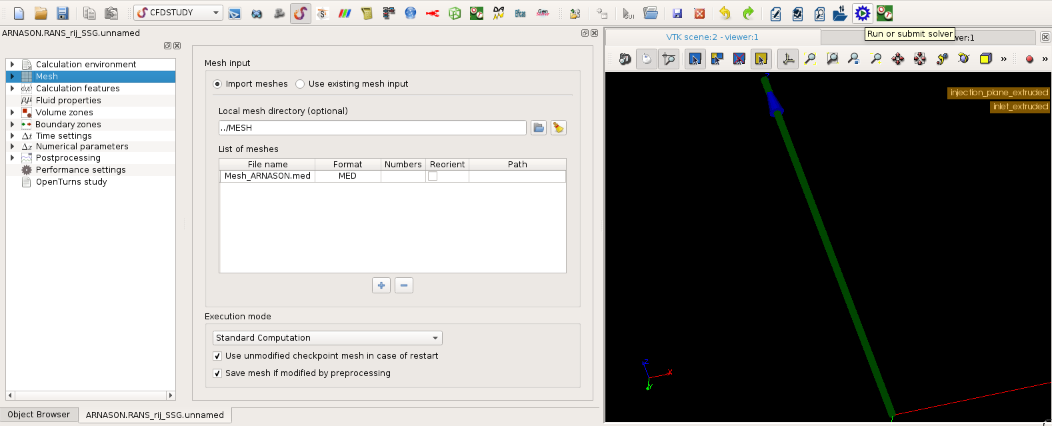
\includegraphics[width=\textwidth]{\IMAGES/Part4_RANS/run_submit_solver.png} 
\caption{Run}
\label{lag:cap1_run}
\end{figure}

A window will open where you can specify the run options.

All options except the number of processes are let to their default values:

\begin{itemize}
\item ‘runcase’ for the ‘Script file’
\item ‘1’ for the number of threads per process
\item build type to '[default]'.
\end{itemize}

Again, you may increase the ‘Number of processes’, depending on the number of cores available on your machine in order to run the simulation in parallel.

\begin{figure}[H]
\centering
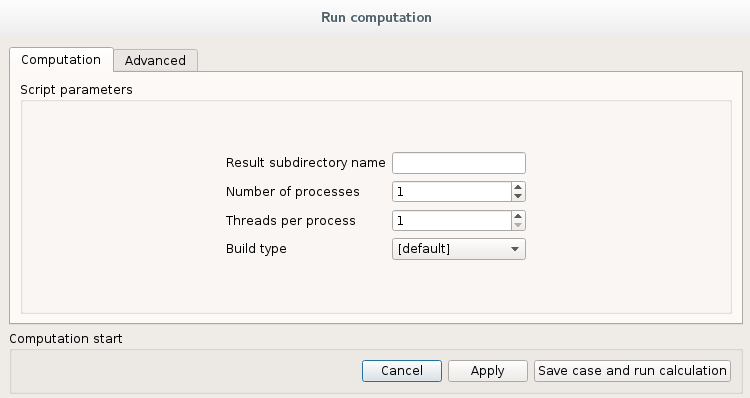
\includegraphics[width=0.7\textwidth]{\IMAGES/Part5_Lagrangian_computation/lagr_nb_proc.png}
\caption{Batch calculation settings.}\label{lag:batch_calculation_setting}
\end{figure}

Press the ‘Save case and run calculation’ button to run \CS.  The pop-up panel for the run opens, listing in real time the different stages of the calculation, from compilation of the user-subroutines to the saving of the results.

\subsection{Post-processing the Results}

For the post-processing of the results, move to the \paravis module.  In the ‘Pipeline Browser’ panel on the left-hand side, right click and select \keys{Open} in the drop-down menu.  Point to the ‘RESULTS.case’ file in the RESU directory for the run that has just finished:

'/../ARNASON/RANS\_rij\_SSG\_5M/RESU/DateOfRunTimeOfRun/postprocessing/RESULTS\\.case'

and to the 'PARTICLES.case' in:

'/../ARNASON/RANS\_rij\_SSG\_5M/RESU/DateOfRunTimeOfRun/postprocessing\\/PARTICLES.case.'

Follow the steps described in tutorials \cite{ShearDriven_Tuto, HeatedDriven_Tuto}, to create the ‘ExtractBlock’ and ‘CellDataPointData’ objects, and post-process the results.


